\section{Filtro pasa-bajos pasivo}

Un filtro pasa-bajos se caracteriza por permitir el paso de señales con frecuencias bajas (relativas a la frecuencia de corte) y atenuar las frecuencias altas. En la siguiente sección se realizará un análisis de su respuesta a señal a distintas frecuencias. 

\subsection{Cálculo y diseño de circuito}

El filtro se compone por un resistor y un capacitor, tomando la salida sobre el último. 

\begin{figure}[H]
	\centering
	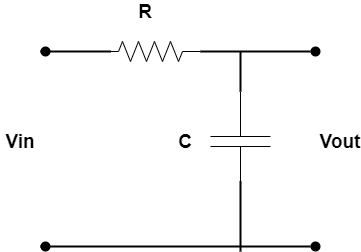
\includegraphics[scale=0.6]{../Informe/Imagenes/RC.png}
	\caption{Esquema filtro pasa bajos}
	\label{ej1cir}
\end{figure}

Se obtiene la función transferencia del sistema empleando un divisor de tensión en $V_0$:

$$\hspace{0.5cm} H(s) = \frac{1}{sCR + 1} $$

Se utilizaron los siguientes valores para los componentes:

\begin{itemize}[leftmargin=2cm]
	\item $R = 1K\Omega$
	\item $C = 10nF$
  \end{itemize}

Reemplazando los valores, se obtiene la función transferencia:

$$\hspace{0.5cm} H(s) = \frac{1}{1\cdot 10^{-5}\cdot s + 1} $$

Cuya frecuencia de corte resulta: $$f_0 = \frac{1}{2\pi RC} \Rightarrow \hspace{0.5cm} f_0 \succeq 15915,5 Hz$$.

Se armó el circuito en el protobard (ver Figura 8). Se empleó un resistor con tolerancia del $5\%$ y un capacitor con tolerancia nominal.

\begin{figure}[H]
	\centering
	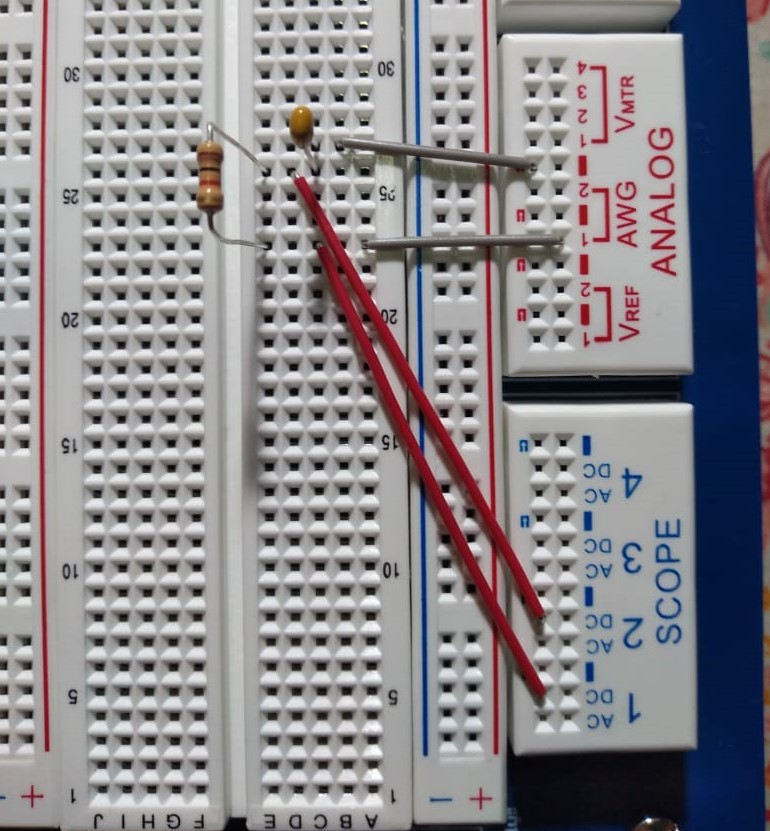
\includegraphics[scale=0.5]{../Informe/Imagenes/RCProto.jpeg}
	\caption{Circuito en protoboard}
	\label{ej1cir}
\end{figure}


\subsection{Respuesta a señal de entrada y análisis a distintas frecuencias}

Se realizó el análisis de la respuesta del circuito a una señal de entrada cuadrada de $6V_pp$ a distintas frecuencias.

Al suministrar la señal cuadrada a una frecuencia de $8kHz$, se puede observar la atenuación de la señal de salida (curva azul, Figura 9), la cual pierde la forma cuadrada y muestra intervalos de caídas y subidas entre los valores absolutos de la tensión suminstrada. La causa de esto se encuentra en la presencia de un capacitor, el cual tiene intervalos de carga y descarga. 

\begin{figure}[H]
	\centering
	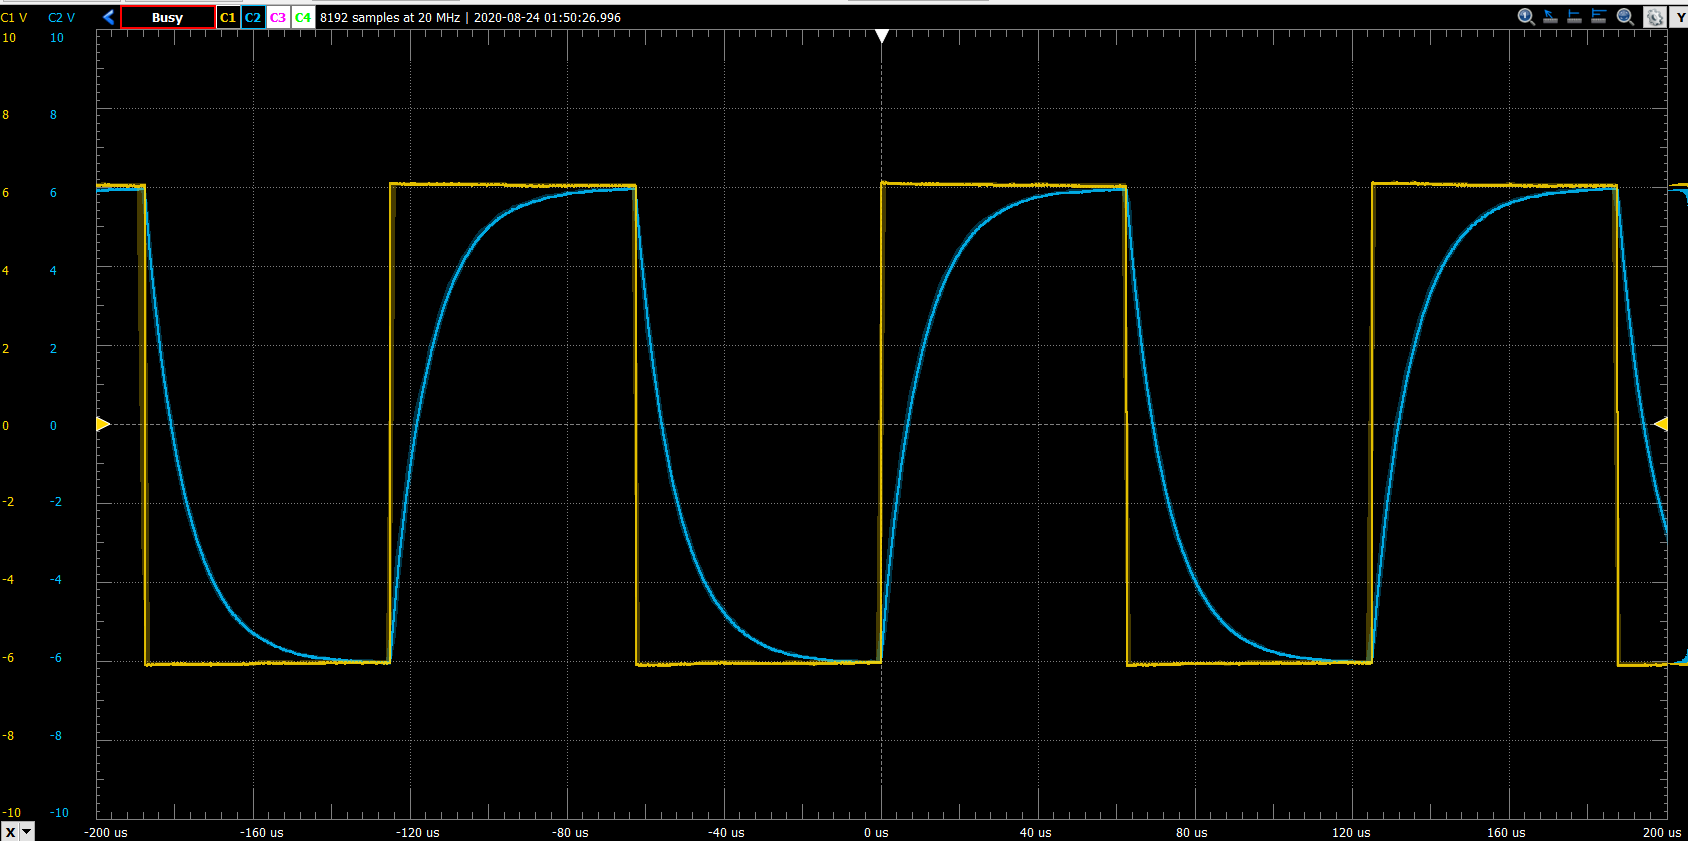
\includegraphics[scale=0.5]{../Informe/Imagenes/Ej2Scope (2).png}
	\caption{Señal de entrada cuadrada de $6V_pp$ a $8kHz$ (amarillo) y señal de salida (azul)}
	\label{ej1cir}
\end{figure}


A 160 Hz, la señal de salida es practicamente igual a la señal de entrada. En este caso, la frecuencia de la señal de entrada esta muy alejada de la frecuencia de corte del sistema. Con estas dos situaciones resulta evidente el accionar de un filtro pasa bajos, permitiendo el paso casi sin afectar a bajas frecuencias respecto a la de corte, y atenuada a frecuencias altas. 

\begin{figure}[H]
	\centering
	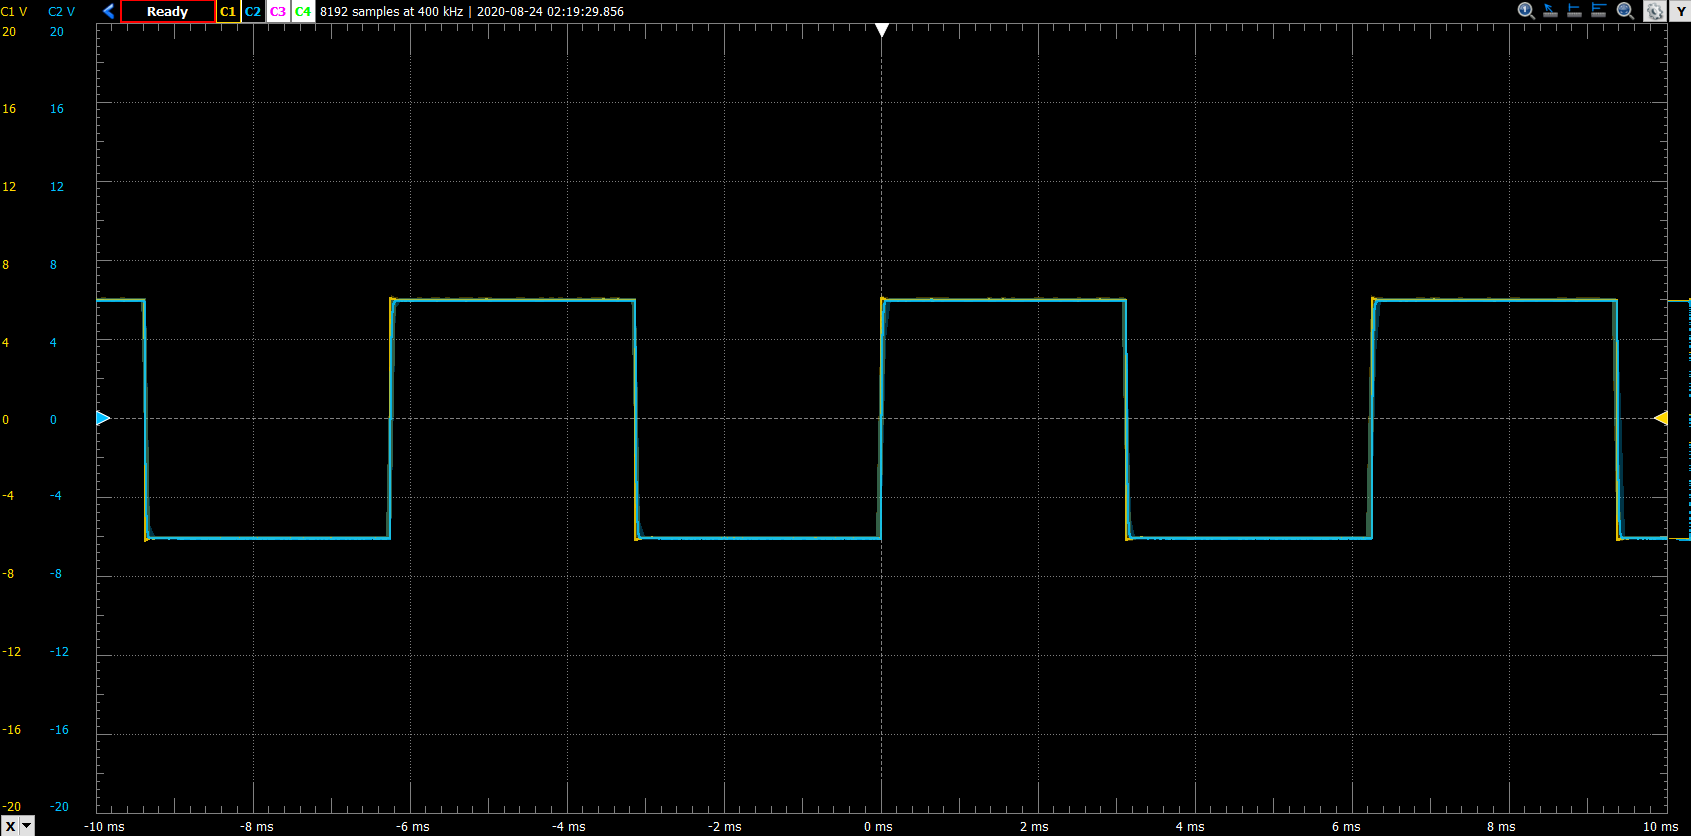
\includegraphics[scale=0.5]{../Informe/Imagenes/Ej2Scope160Hz (2).png}
	\caption{Señal de entrada cuadrada de $6V_pp$ a $160Hz$ (amarillo) y señal de salida (azul)}
	\label{ej1cir}
\end{figure}


Un análisis de los armónicos (componentes) de la señal de entrada y de salida del sistema permite visualizar las características del mismo. 

$$ x(t) = \begin{cases} -A &\mbox{si } \frac{T}{2}\leq t\leq 0\\
    A & \mbox{si } 0\leq t\leq \frac{T}{2}\end{cases} \pmod{2}. $$

Si se piensa en su serie trigonométrica de Fourier:

$$ x(t)=a_{0}+\sum_{1}^{\infty}\ a_{n}cos(\frac{2\pi nt}{T}) +b_{n}\sin(\frac{2\pi nt}{T}) $$

Luego, $a_0$ = $a_n$ = 0 por ser función impar. Calculando los coeficientes $b_n$ se obtiene:

$$b_{n} =\frac{2}{T}\int_{-\frac{T}{2}}^{\frac{T}{2}}x(t)\sin (\frac{2\pi nt}{T}) = \frac{4}{T}\int_{0}^{\frac{T}{2}}A\sin (\frac{2\pi nt}{T})=-2A\left [ \frac{\left ( -1 \right )^{n}-1}{n\pi } \right ]$$


$$ b_{n} = \begin{cases} 0 &\mbox{si } n par\\
    \frac{4A}{n\pi} & \mbox{si } n impar\end{cases} \pmod{2}. $$


Teniendo en cuenta la relación entre los coeficientes de la serie exponencial y trigonométrica de Fourier y considerando que A = 3, obtengo los coefiecientes de la serie exponencial:

$$ X_{n}=\frac{j2A}{(2n+1)\pi } = \frac{j6}{(2n+1)\pi } $$

Dada la relación $Y(f)$ = $H(f)X(f)$, como se trata de un sistema LTI (lo vemos en la H(s)) y teniendo en cuenta que $s$ = $j2\pi$$f$, luego se pueden obtener los coeficientes de la señal de salida como:

$$Y_{n} = H(f_{0}(2n+1))X_{n}$$

Siendo los coeficientes de la serie exponencial de Fourier de la señal de salida:

$$Y_{n} = \frac{6j}{(j2\pi f_{0}(2n+1)RC +1) (j\pi (2n+1))}$$

Considerando los módulos de los coeficientes de la SEF:

$$\left | X_{n} \right | = \frac{6}{(2n+1)\pi }$$

$$\left | Y_{n} \right | = \frac{6j}{\sqrt{(j2\pi^{2} f_{0}(2n+1)^{2}RC)^{2} +\pi^{2}(2n+1)^{2})}}$$

De la expresión del módulo de los coeficientes de la SEF de la señal de salida se puede observar que a mayor frecuencia, el denominador es mayor y el módulo es cada vez menor. Comparando las expresiones de $X_n$ e $Y_n$ se ve que el filtro produce una atenuación de la señal, siendo notorios los efectos al aumentar la frecuencia $f_0$.

\begin{figure}[H]
	\centering
	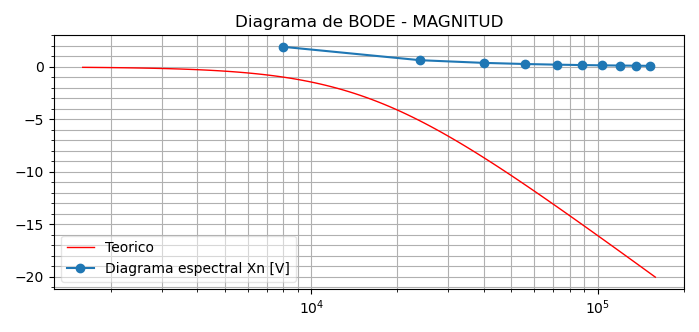
\includegraphics{../Informe/Imagenes/BodeEj2.png}
	\caption{Diagrama de Bode: Ganancia (en dB) superpuesta con diagrama espectral de señal de entrada (en V) $f_0$ = 8kHz}
	\label{ej1cir}
\end{figure}

En la Figura 11 se superpuso el gráfico de ganancia del diagrama de Bode (teorico y medido) con el diagrama espectral en amplitud de la SEF de la señal de entrada (los puntos aparecen unidos). Se puede observar una rápida caída de la amplitud apenas con los primeros armónicos, ubicándose además la mayoría en la zona de mayor atenuación. Al estar los armónicos en la zona de frecuencias por encima de la frecuencia de corte, la señal de salida que se formará dificilmente adopte la forma de una señal cuadrada como la de la entrada (recordemos que al expresar una función como suma de senos y cosenos o exponenciales, a mayor cantidad de términos mas se aproximará a la señal original).

\begin{figure}[H]
	\centering
	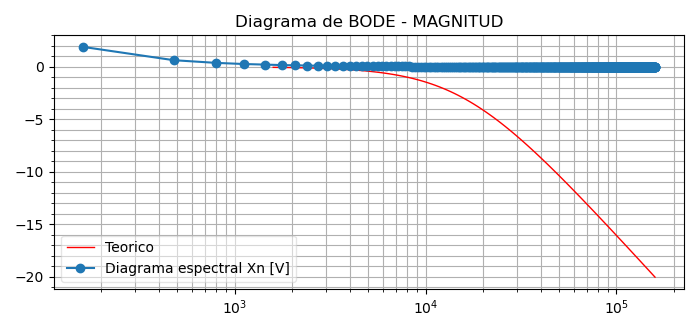
\includegraphics{../Informe/Imagenes/Bode160Hz.png}
	\caption{Diagrama de Bode: Ganancia (en dB) superpuesta con diagrama espectral de señal de entrada (en V) a una $f_0$ = 160Hz}
	\label{ej1cir}
\end{figure}

En la Figura 12, en tanto, se observa que a una $f_0$ = 160Hz una gran parte de los armónicos se ubican por debajo de la frecuencia de corte (zona de poca caída en la ganancia), lo que permite que la expresión de la señal de salida tenga mas términos y se aproxime a la señal de entrada. Esto se pudo corroborar al observar la señal de salida a frecuencia. Se verifica de ambas $f_0$ que las componentes de la señal de entrada de mas alta frecuencia son atenuados por el filtro.


Si se eleva la frecuencia de la señal de entrada muy por encima de la frecuencia de corte, se tiene que el término $sRC\gg 1$ y la función de transferencia del circuito se aproxima a:

$$H(s)= \frac{1}{s}$$

Esta expresión de H(s) podría pensarse como un 'integrador', debido a que al obtener la señal de salida se estaría "integrando", pensando en la transformada de Laplace, la señal de entrada.

Para verificarlo, se sometió al circuito a una señal de entrada de 150kHz, unas 10 veces mas que la frecuencia de corte, observandose en la salida (ver Figura 13) una señal aproximadamente triangular, resultado que corresponde con lo esperado. 

\begin{figure}[H]
	\centering
	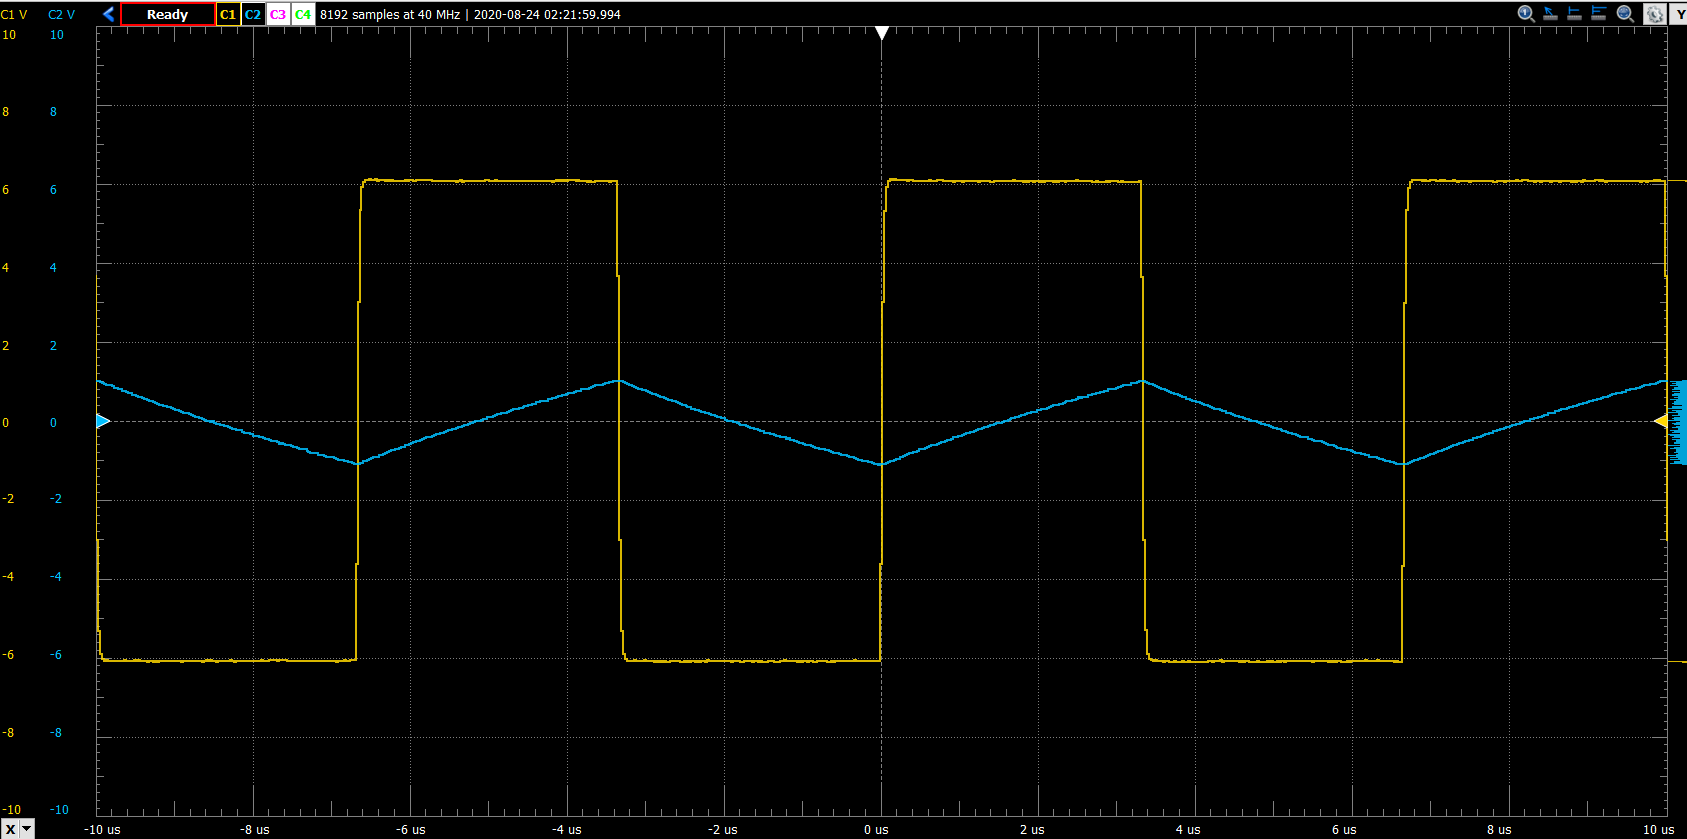
\includegraphics[scale=0.5]{../Informe/Imagenes/Ej2Scope150kHz (2).png}
	\caption{Señal de entrada cuadrada de $6V_pp$ a $150kHz$ (amarillo) y señal de salida (azul)}
	\label{ej1cir}
\end{figure}